\documentclass[twocolumn]{bmcart}% uncomment this for twocolumn layout and comment line below
%% BioMed_Central_Tex_Template_v1.06
%%                                      %
%  bmc_article.tex            ver: 1.06 %
%                                       %

%%IMPORTANT: do not delete the first line of this template
%%It must be present to enable the BMC Submission system to
%%recognise this template!!

%%%%%%%%%%%%%%%%%%%%%%%%%%%%%%%%%%%%%%%%%
%%                                     %%
%%  LaTeX template for BioMed Central  %%
%%     journal article submissions     %%
%%                                     %%
%%          <8 June 2012>              %%
%%                                     %%
%%                                     %%
%%%%%%%%%%%%%%%%%%%%%%%%%%%%%%%%%%%%%%%%%


%%%%%%%%%%%%%%%%%%%%%%%%%%%%%%%%%%%%%%%%%%%%%%%%%%%%%%%%%%%%%%%%%%%%%
%%                                                                 %%
%% For instructions on how to fill out this Tex template           %%
%% document please refer to Readme.html and the instructions for   %%
%% authors page on the biomed central website                      %%
%% http://www.biomedcentral.com/info/authors/                      %%
%%                                                                 %%
%% Please do not use \input{...} to include other tex files.       %%
%% Submit your LaTeX manuscript as one .tex document.              %%
%%                                                                 %%
%% All additional figures and files should be attached             %%
%% separately and not embedded in the \TeX\ document itself.       %%
%%                                                                 %%
%% BioMed Central currently use the MikTex distribution of         %%
%% TeX for Windows) of TeX and LaTeX.  This is available from      %%
%% http://www.miktex.org                                           %%
%%                                                                 %%
%%%%%%%%%%%%%%%%%%%%%%%%%%%%%%%%%%%%%%%%%%%%%%%%%%%%%%%%%%%%%%%%%%%%%

%%% additional documentclass options:
%  [doublespacing]
%  [linenumbers]   - put the line numbers on margins

%%% loading packages, author definitions

%\documentclass[twocolumn]{bmcart}% uncomment this for twocolumn layout and comment line below
%\documentclass{bmcart}

%%% Load packages
\usepackage{amsthm,amsmath}
%\RequirePackage{natbib}
%\RequirePackage[authoryear]{natbib}% uncomment this for author-year bibliography
%\RequirePackage{hyperref}
\usepackage[utf8]{inputenc} %unicode support
%\usepackage[applemac]{inputenc} %applemac support if unicode package fails
%\usepackage[latin1]{inputenc} %UNIX support if unicode package fails
\usepackage{graphicx}
\usepackage{lipsum}

%%%%%%%%%%%%%%%%%%%%%%%%%%%%%%%%%%%%%%%%%%%%%%%%%
%%                                             %%
%%  If you wish to display your graphics for   %%
%%  your own use using includegraphic or       %%
%%  includegraphics, then comment out the      %%
%%  following two lines of code.               %%
%%  NB: These line *must* be included when     %%
%%  submitting to BMC.                         %%
%%  All figure files must be submitted as      %%
%%  separate graphics through the BMC          %%
%%  submission process, not included in the    %%
%%  submitted article.                         %%
%%                                             %%
%%%%%%%%%%%%%%%%%%%%%%%%%%%%%%%%%%%%%%%%%%%%%%%%%


%\def\includegraphic{}
%\def\includegraphics{}



%%% Put your definitions there:
\startlocaldefs
\endlocaldefs


%%% Begin ...
\begin{document}

%%% Start of article front matter
\begin{frontmatter}

\begin{fmbox}
\dochead{Software}

%%%%%%%%%%%%%%%%%%%%%%%%%%%%%%%%%%%%%%%%%%%%%%
%%                                          %%
%% Enter the title of your article here     %%
%%                                          %%
%%%%%%%%%%%%%%%%%%%%%%%%%%%%%%%%%%%%%%%%%%%%%%

\title{Recursive Dynamic Markov Clustering for fine-grained orthogroup classification}

%%%%%%%%%%%%%%%%%%%%%%%%%%%%%%%%%%%%%%%%%%%%%%
%%                                          %%
%% Enter the authors here                   %%
%%                                          %%
%% Specify information, if available,       %%
%% in the form:                             %%
%%   <key>={<id1>,<id2>}                    %%
%%   <key>=                                 %%
%% Comment or delete the keys which are     %%
%% not used. Repeat \author command as much %%
%% as required.                             %%
%%                                          %%
%%%%%%%%%%%%%%%%%%%%%%%%%%%%%%%%%%%%%%%%%%%%%%

\author[
   addressref={aff1},                    % id's of addresses, e.g. {aff1,aff2}
   %noteref={n1},                        % id's of article notes, if any
   %corref={aff1},                       % id of corresponding address, if any
   %email={steve.bond@nih.gov}            % email address
]{\inits{SR}\fnm{Stephen R} \snm{Bond}}
\author[
   addressref={aff1},
   %email={karlkeat@gmail.com}
]{\inits{P}\fnm{Paul} \snm{Gonzalez}}
\author[
   addressref={aff1},
   %email={karlkeat@gmail.com}
]{\inits{KE}\fnm{Karl E} \snm{Keat}}
\author[
   addressref={aff1},
   email={andy@mail.nih.gov}
]{\inits{AD}\fnm{Andreas D} \snm{Baxevanis}}
%%%%%%%%%%%%%%%%%%%%%%%%%%%%%%%%%%%%%%%%%%%%%%
%%                                          %%
%% Enter the authors' addresses here        %%
%%                                          %%
%% Repeat \address commands as much as      %%
%% required.                                %%
%%                                          %%
%%%%%%%%%%%%%%%%%%%%%%%%%%%%%%%%%%%%%%%%%%%%%%

\address[id=aff1]{%                           % unique id
  \orgname{Computational and Statistical
   Genomics Branch, Division of Intramural    % university, etc
    Research, National Human Genome
     Research Institute, National
      Institutes of Health},
  \street{50 South Drive},                     %
  \postcode{20892}                             % post or zip code
  \city{Bethesda},                             % city
  \state{MD},
  \cny{USA}                                    % country
}

%%%%%%%%%%%%%%%%%%%%%%%%%%%%%%%%%%%%%%%%%%%%%%
%%                                          %%
%% Enter short notes here                   %%
%%                                          %%
%% Short notes will be after addresses      %%
%% on first page.                           %%
%%                                          %%
%%%%%%%%%%%%%%%%%%%%%%%%%%%%%%%%%%%%%%%%%%%%%%

%\begin{artnotes}
%\note{Sample of title note}     % note to the article
%\note[id=n1]{Equal contributor} % note, connected to author
%\end{artnotes}

%\end{fmbox}% comment this for two column layout

%%%%%%%%%%%%%%%%%%%%%%%%%%%%%%%%%%%%%%%%%%%%%%
%%                                          %%
%% The Abstract begins here                 %%
%%                                          %%
%% Please refer to the Instructions for     %%
%% authors on http://www.biomedcentral.com  %%
%% and include the section headings         %%
%% accordingly for your article type.       %%
%%                                          %%
%%%%%%%%%%%%%%%%%%%%%%%%%%%%%%%%%%%%%%%%%%%%%%

\begin{abstractbox}

\begin{abstract} % abstract
\parttitle{Background}  % Required
Blahh

\parttitle{Results}  % Required
Blahh

\parttitle{Conclusions}  % Required
Blahh

\end{abstract}

%%%%%%%%%%%%%%%%%%%%%%%%%%%%%%%%%%%%%%%%%%%%%%
%%                                          %%
%% The keywords begin here                  %%
%%                                          %%
%% Put each keyword in separate \kwd{}.     %%
%%                                          %%
%%%%%%%%%%%%%%%%%%%%%%%%%%%%%%%%%%%%%%%%%%%%%%

\begin{keyword}  % Three to ten keywords
\kwd{orthogroup}
\kwd{ortholog}
\kwd{Markov clustering}
\end{keyword}

% MSC classifications codes, if any
%\begin{keyword}[class=AMS]
%\kwd[Primary ]{}
%\kwd{}
%\kwd[; secondary ]{}
%\end{keyword}

\end{abstractbox}
%
\end{fmbox} % uncomment this for twcolumn layout

\end{frontmatter}

%%%%%%%%%%%%%%%%%%%%%%%%%%%%%%%%%%%%%%%%%%%%%%
%%                                          %%
%% The Main Body begins here                %%
%%                                          %%
%% Please refer to the instructions for     %%
%% authors on:                              %%
%% http://www.biomedcentral.com/info/authors%%
%% and include the section headings         %%
%% accordingly for your article type.       %%
%%                                          %%
%% See the Results and Discussion section   %%
%% for details on how to create sub-sections%%
%%                                          %%
%% use~\cite{...} to cite references        %%
%% ~\cite{koon} and                         %%
%% ~\cite{oreg,khar,zvai,xjon,schn,pond}    %%
%%  \nocite{smith,marg,hunn,advi,koha,mouse}%%
%%                                          %%
%%%%%%%%%%%%%%%%%%%%%%%%%%%%%%%%%%%%%%%%%%%%%%

%%%%%%%%%%%%%%%%%%%%%%%%% start of article main body
% <put your article body there>

%%%%%%%%%%%%%%%%
%% Background %%
%%
\section{Background}\label{sec:background}
When a gene evolves an important physiological function, purifying selection tends to maintain that function through evolutionary time~\cite{Altenhoff:2012ea, KryuchkovaMostacci:2016iw, Rogozin:2014fp}.
As a result, orthology (i.e., homology via speciation) has become a widely used predictor of shared gene product function among species, and considerable effort has been made to develop computational tools for identifying orthologs from genomic data.
Due to the non-transitive nature of orthology (i.e., paralogs in one species can be orthologous to a single gene in another species), grouping pure sets of one-to-one orthologs is often not possible~\cite{Fitch:2000tf}.
Instead, the term `orthogroup' has come to represent a cluster of genes descended from a common ancestor of the clade in question, which may include paralogs~\cite{Wapinski:2007fa}.
The algorithms currently in popular use for defining orthogroups fall into three broad categories: Synteny-based, tree-based, and graph-based clustering methods (recently reviewed in~\cite{Tekaia:2016ga} and~\cite{Habermann2016}).

Syntenic neighborhoods degrade rapidly with evolutionary distance, so pure synteny-based approaches are not generally appropriate except between closely related taxa~\cite{Kristensen:2011gw}.
Furthermore, such approaches require highly contiguous genomic assemblies;
while advances in long-read sequencing technology and de novo assembly will likely allow future genome sequencing efforts to achieve the necessary standards, current genome projects often remain highly fragmented~\cite{Koren:2015il}.

Tree-based approaches (e.g., Ensembl Compara~\cite{Vilella:2009ju}, LOFT~\cite{vanderHeijden:2007bo}, and SYNERGY~\cite{Wapinski:2007fa}) identify orthologous clades by estimating phylogenetic trees for a target gene family, and then attempt to reconcile those gene trees against a `known' species tree.
The accuracy of tree-based orthology prediction methods is tied closely to the accuracy of the species trees they rely on;
this can lead to considerable uncertainty or error, especially for less well-studied taxonomic groups~\cite{Xu:2016ek}.

Finally, pairwise similarity methods leverage graph theory to rapidly identify groups of related sequences.
InParanoid~\cite{OBrien:2005cy}, EggNOG~\cite{Jensen:2007cc}, and OMA~\cite{Roth:2009iu} are popular tools for assigning sequences to orthogroups using a `best-hit clique' approach, where closed best-hit sub-graphs are identified in the dataset.
These methods can be fast and accurate for detecting one-to-one orthologs, but they suffer diminishing recall rates when in-paralogs are present among the species under study~\cite{Dalquen:2013fz} (`in-paralog' describes homologs derived from genetic duplication \textit{after} speciation~\cite{Sonnhammer:2002vm,Tekaia:2016ga}).
In contrast, Markov clustering (MCL) can efficiently isolate more inclusive sub-graphs~\cite{VanDongen:kJZ890qx,Enright:2002uq}, although the trade-off is generally a reduction in precision;
it is often difficult to separate closely related orthogroups within a given gene family.
Indeed, the major challenge facing those wishing to analyze a defined gene family is \textit{resolution}, because the popular MCL-based ortholog prediction methods, such as OrthoMCL~\cite{Li:2003en}, OrthoFinder~\cite{Emms:2015ig}, and ProteinOrtho~\cite{Lechner:2011jk}, are targeted towards coarse-grained clustering of all protein models derived from whole-genome data.
While computationally efficient, these resources are not well suited for fine-grained processing of individual gene families where all input sequences are homologous.
This leaves a gap in our ability to easily discern evolutionary patterns at this scale and has inevitably exacerbated the propagation of annotation errors in our public databases~\cite{Schnoes:2009gb}, which still relies heavily on annotation transfer following inference of homology against a limited number of reference species~\cite{Aken:2016dl, Mi:2016bw, OLeary:2016cm}.
Here we present a method that overcomes these challenges, along with a suite of tools to assist with detailed downstream analysis.


\section{Results and Discussion}\label{sec:resultsAndDiscussion}
Recursive Dynamic Markov Clustering (RD-MCL) is a new pairwise similarity graph-based orthogroup prediction heuristic that achieves high precision within the context of a gene family.
Specifically, RD-MCL significantly improves upon the BLASTP-based pairwise similarity metrics currently in popular use, applies an optimization algorithm to dynamically select MCL parameters, recursively subdivides overly inclusive orthogroups, and implements final polishing steps to maximize overall accuracy (Figure~\ref{fig:pipeline}).
The entire workflow has been encapsulated in a single executable, which can be run from the command line and minimally requires a sequence file as input.
Given sufficient taxonomic coverage, RD-MCL clearly reveals mis-assembled or mis-annotated sequences, as well as orthogroups that have been previously undescribed.
Furthermore, a set of high quality orthogroups from a well-sampled taxonomic group can be leveraged to analyze sequences from clades that are less well sampled, allowing for detailed phylogenetic placement of new sequences into a gene family with greater precision than is possible with simple best-hit database queries.
The software is open-source (https://research.nhgri.nih.gov/software/RD-MCL/) and distributed as part of a suite of tools to facilitate all of the downstream analyses reported here.

\begin{figure*}[t]
  \begin{center}
  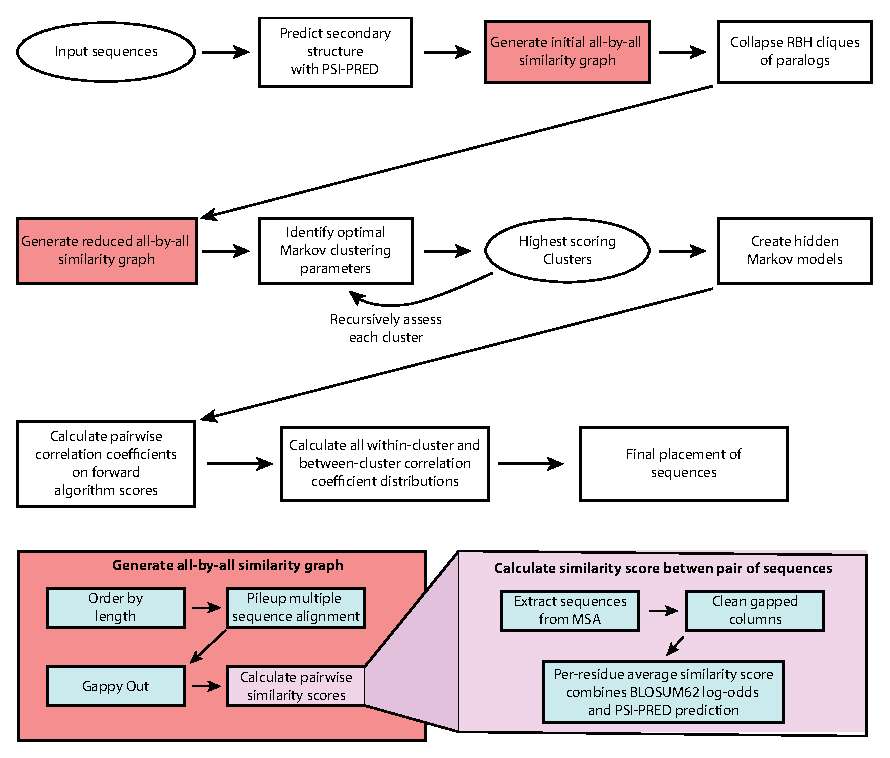
\includegraphics[height=0.6\textheight]{../figures/pipeline.eps}
\end{center}
\caption{Pipeline.}
\label{fig:pipeline}
\end{figure*}

\subsection{Overcoming BLAST-based similarity metric limitations}\label{subsec:overcomingBlast-basedSimilarityMetricLimitations}
BLASTP scores reduce overall resolving power of MCL when sequences are too similar or too dissimilar.
BLAST scores (bit or e-value) have a strong length bias when calculating orthogroups, but this can be corrected for by creating a linear model from the top 5\% of matches between two species and scaling all other matches according to that model~\cite{Emms:2015ig}.
OrthoFinder also uses a static inflation/edge similarity threshold for MCL~\cite{Emms:2015ig}

Need a figure that illustrates relative information content of each metric.

\subsection{MCL parameters must be tuned to maximally resolve orthogroups}\label{subsec:mclParametersMustBeTunedToMaximallyResolveOrthogroups}
\lipsum[1]

\subsection{Recursive MCL compensates for variable evolutionary separation within and between orthogroups}\label{subsec:recursiveMclCompensatesForVariableEvolutionarySeparationBetweenOrthogroups}
\lipsum[1]

\subsection{Simulation data across the dynamic range of RD-MCL}\label{subsec:simulationDataAcrossTheDynamicRangeOfRd-mcl}
To test the performance of RD-MCL compared to other available ortholog prediction tools, we simulated sets of homologs using the Pyvolve module~\cite{Spielman:2015kv}.
These simulations varied in the number of sequences, branch length (substitutions per site), degree of gene loss or duplication, and domain architecture.
The initial seed sequence for all simulations was a polypeptide 398 amino acids long containing four transmembrane domains.
More extensive descriptions of the following simulations can be found in the Methods section.

OrthoFinder performs extremely poorly, but this is probably due to the scaling factor that it generates when classifying orthogroups.
We are not providing enough data to generate a productive linear model~\cite{Emms:2015ig}.
Is it worth while to create a ven diagram illustrating the overlap between methods?

\subsubsection{Branch lengths}
Given an idealized set of homologous sequences, where there has been no gene loss and all gene duplications occurred prior to the last common ancestor of the taxa included in the set, the phylogenetic relationship within each orthogroup should closely approximate the underlying species tree.
Furthermore, the phylogenetic relationship among the orthogroups will approximate the original gene tree of all paralogs present in the last common ancestor.
As such, two distinct axes of divergence must be accounted for when assessing the effect of branch length (i.e., substitutions per site), which we will refer to as the 'species tree length' and 'gene tree length', respectively.

% Maybe make a figure here, to show the two axes of divergence??

A total of 625 datasets were simulated, with each containing eight taxa and seven orthologs (for 56 sequences per dataset).
Branch lengths were varied from 0.05 to 1.55 substitutions per site with standard deviations between 0.05 and 1.05 to prevent perfectly symetrical trees.
As illustrated in Figure~\ref{fig:branch_len_3d}, RD-MCL was either equivalent to or out performed OrthoFinder, OrthoMCL, and ProteinOrtho across the entire dynamic range assessed.
All of the methods tested were more sensitive to changes in species tree branch lengths than they were to gene tree branch lengths (i.e., branches within an orthogroup, as opposed to between orthogroups), although both RD-MCL and OrthoMCL performed marginally better on short species trees with the gene trees were longer.

% May_3_2017_orthofinder_branch_lengths/orthofinder_BL.ipynb
% May_3_2017_OrthoMCL_branch_lengths/orthomcl_BL.ipynb
% May_3_2017_proteinortho_branch_lengths/proteinortho_bl.ipynb
% May_3_2017_rdmcl_branch_len/rdmcl_BL.ipynb
\begin{figure}[t]
  \begin{center}
  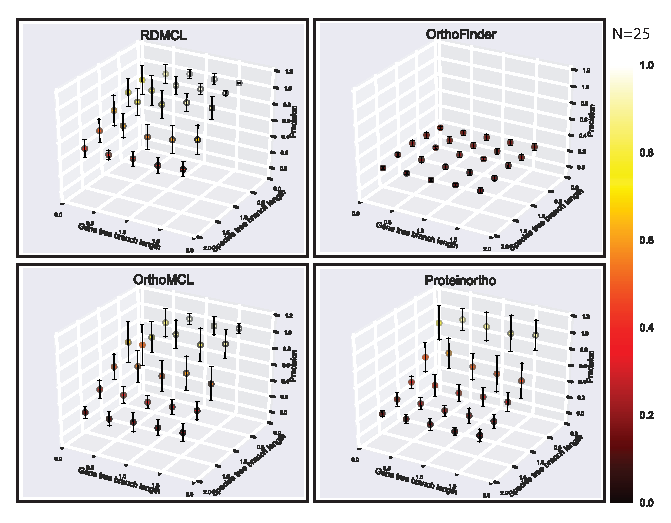
\includegraphics[height=0.25\textheight]{../figures/branch_len_3D_scatter.eps}
\end{center}
\caption{Effect of branch length on precision of orthogroup prediction.}
\label{fig:branch_len_3d}
\end{figure}

Figure~\ref{fig:branch_len_std} illustrates the case-by-case performance of RD-MCL compared to the other methods by standardizing the relative precision achieved on each dataset against the precision of RD-MCL\@.

% May_03_2017_branch_lengths.ipynb
\begin{figure}[t]
  \begin{center}
  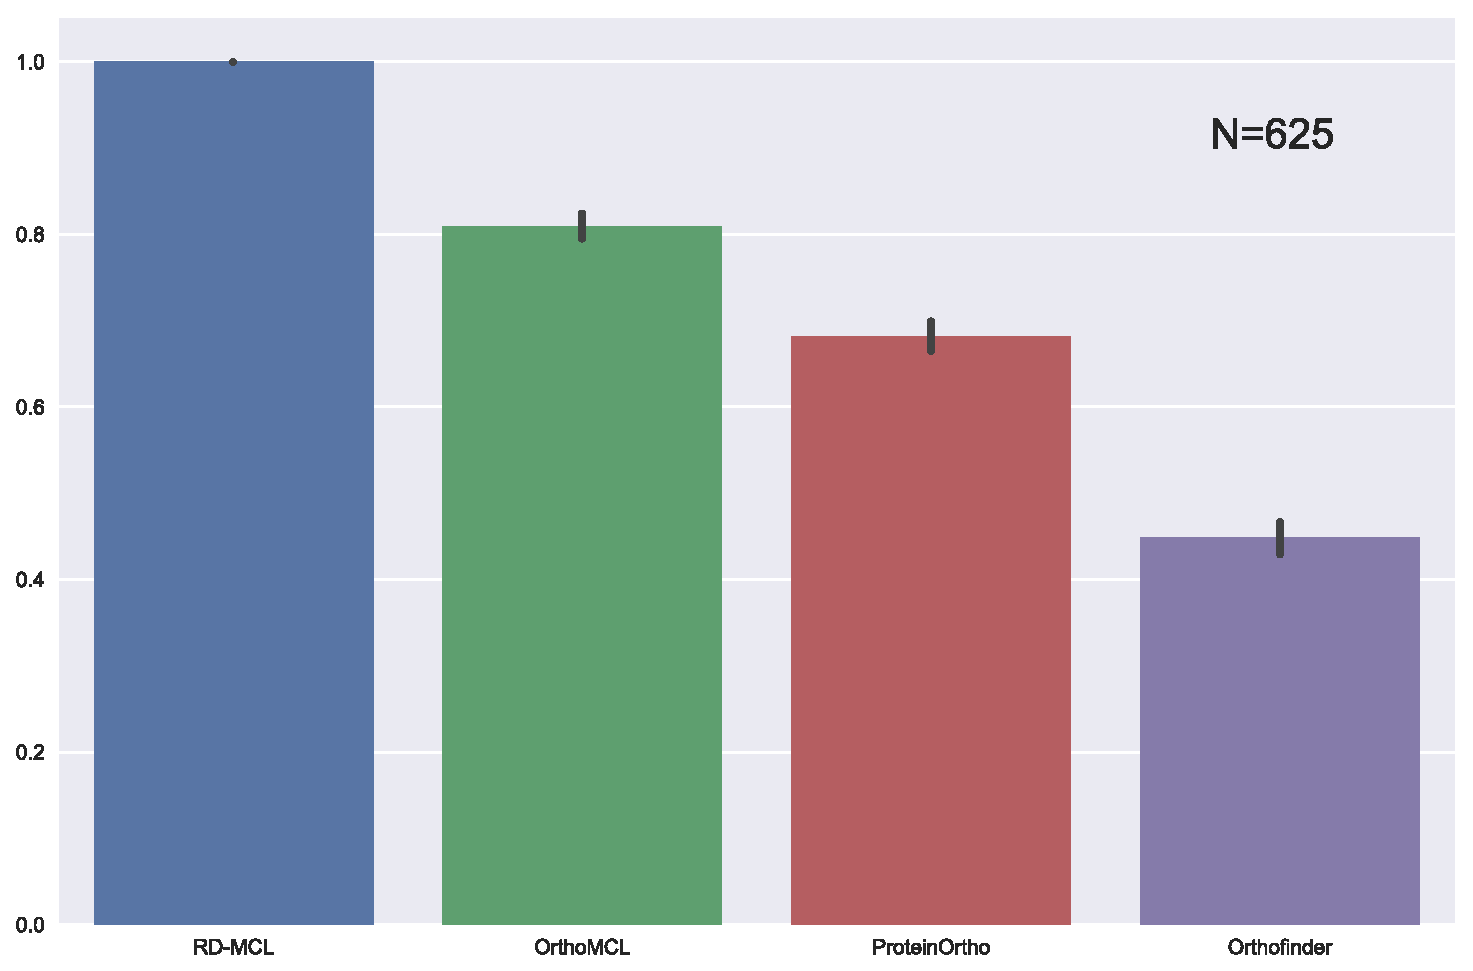
\includegraphics[height=0.22\textheight]{../figures/branch_len_bargraph.eps}
\end{center}
\caption{Effect of branch length on precision of orthogroup prediction.}
\label{fig:branch_len_std}
\end{figure}

\subsubsection{Number of sequences}
To test the effects of increasing the number of orthogroups and orthogroup size, datasets were simulated with 4 to 30 taxa and between 4 and 30 genes per taxa.

\subsubsection{Missing data}
\lipsum[1]

\subsubsection{Gene duplications}
\lipsum[1]

\subsubsection{Hybrid sequences (weird domain structures)}
\lipsum[1]

\subsection{RD-MCL classification of sample gene families}\label{subsec:rd-mclClassificationOfSampleGeneFamilies}
\lipsum[1]

\subsubsection{Caspases: Recovering known orthogroups from well sampled clades}
Caspases are cysteine-dependent aspartyl-specific proteases with key regulatory roles in inflammation, immunity, and tissue homeostasis~\cite{Songane:2018kq, McIlwain:2013iy}.
The complement of chordate caspases has been well described, often through careful reconstruction of genomic synteny, along with a rich history of gene duplications and losses in specific clades~\cite{Eckhart:2008gv, Sakamaki:2009fu, Sakamaki:2015kb, Sakata:2007bs}.

Discuss the mess that is Casps-1/4/5/12/13

\subsubsection{WNTs: Anchoring novel orthogroups from transcriptome date}
\lipsum[1]

\subsection{Downstream analyses}\label{subsec:downstreamAnalyses}
\subsubsection{Inferring orthogroup 'gene-trees' from consensus sequences}
\lipsum[1]

\subsubsection{Inferring species trees from RD-MCL generated orthogroups}
\lipsum[1]

\subsubsection{Phylogenetic placement of new genes into pre-calculated orthogroups}
\lipsum[1]

\subsection{Implementation}\label{subsec:implementation}
RD-MCL has been implemented in Python with a command-line interface

Python is not generally well adapted for distributing complex operations across a cluster environment, but creating all-by-all similarity graphs is an O\textsuperscript{2} hard problem that makes RD-MCL run times prohibitive when analyzing more than a few hundred sequences on a single machine.
To overcome this challenge, similarity graph creation can be passed off to worker processes which control other nodes on a cluster.
This dynamic is achieved by writing job information to a SQLite database that is monitored by the worker nodes, which then further subdivide the work if a graph is large, and return the results to the same SQLite database for retrieval by the master process.
By distributing the work in this fashion, an arbitrary number of RD-MCL runs can all access the same pool of worker nodes, and the size of the worker pool can be modified on the fly.

Sequence handling is achieved with BuddySuite~\cite{Bond:2017bj}.

\section{Conclusions}\label{sec:conclusions}
It is important to remember that true orthologs are not intrinsically special.
While negative selection is a strong strong evolutionary pressure that tends to preserve function among orthologs, the fate of any given gene is still at the mercy of biological context and the stochastic nature of inheritance.
Therefore, it can be more appropriate to focus on hierarchical similarity among proteins than on their actual genealogy.

\section{Methods}\label{sec:methods}
\subsection{Simulation data}\label{subsec:simulationData}
The performance of each tool was assessed by calculating the precision and recall of the result on simulated data~\cite{Emms:2015ig}.

\begin{gather*}
    Precision = \frac{TP}{TP + FP}\\
    \\
    Recall = \frac{TP}{TP + FN}\\
    \\
    F Score = 2 * \frac{precision * recall}{precision + recall}\\
\end{gather*}

Where TP is True Positive, FP is False Positives, and FN is False Negatives.

\subsection{Caspase and WNT sequence data}\label{subsec:caspaseAndWntSequenceData}
The CASc domain from human caspase-2 (NCBI accession NP\_116764.2) and the wnt domain from mouse Wnt-6 (UniProt accession AAA40569.1) were each used as the starting sequence for a three-iteration PSI-BLAST search of the RefSeq database, limiting the results to metazoans (taxid: 33208), an expectation threshold of 0.01, and allowing for the return of up to 20,000 target sequences.
Accession numbers for all target sequences were downloaded directly from the PSI-BLAST results page, then DatabaseBuddy~\cite{Bond:2017bj} was used to filter out isoforms, partial sequences, and low-quality sequences before fetching the GenBank records.
Given the current depth of species-level coverage in RefSeq, five taxonomic ranges were identified as most appropriate for input into RD-MCL: \textit{Actinopterygii}, \textit{Achelosauria}, \textit{Mammalia}, \textit{Diptera}, and \textit{Hymenoptera}.
The transcriptomes of 25 cnidarian species~\cite{Zapata:2015cc}, assembled using TransDecoder.LongOrfs V.3.0.1~\cite{Haas:2013jq}, were also queried for WNT sequences using BLASTP\@.
These sequences were combined with those cnidarian sequences identified in RefSeq for \textit{Cnidaria}-specific RD-MCL analysis.

\subsection{RD-MCL fitness function}\label{subsec:rd-mclFitnessFunction}
Putative orthogroups were assigned a score based on the size and composition of the cluster, as well as the entire population of sequences available.

Let each sequence $s$ be an element of a set $T$ where all sequences come from the same taxon $j$.

\[
T_j = \{s:s \text{ is a gene in } j\}
\]

All sequences are assigned a score $S$, which is scaled against the largest set of sequences, $T^*$, to bound the minimum score at 1.

\begin{gather*}
    T^* = T_j:|T_j| = max(|T|)\\
    \\
    S_j = \frac{|T^*|}{|T_j|}\\
\end{gather*}

Doing so gives greater weight to those species which have not experienced additional gene expansion, thus allowing greater inclusion of paralogs from those species where gene expansion has been more common.

To penalize the inclusion of paralogs in a putative orthogroup $O$, a diminishing returns algorithm was implemented.
Sequences in the cluster are first sorted into the fewest number of subsets, of largest possible size, where each taxon is represented only once.
This can be expressed as a matrix of size $X \times Y$, where $X$ is the total number of unique taxa and $Y$ is the largest number of sequences derived from a single taxon in the given set.
Each column therefore represents a taxon and is filled from the top down with $S_j$ for each gene it contains, followed by zeros.
For example:


\[
O \equiv
\begin{bmatrix}
    S_{j_1} & S_{j_2} & S_{j_3} & S_{j_4} & S_{j_5} & 0 & S_{j_7}\\
    0 & S_{j_2} & 0 & S_{j_4} & 0 & 0 & S_{j_7} \\
    0 & S_{j_2} & 0 & S_{j_4} & 0 & 0 & 0 \\
    0 & S_{j_2} & 0 & 0 & 0 & 0 & 0 \\
\end{bmatrix}
\]

Each row $Y$ is summed and modified by cofactors $\psi$ and $\gamma$. $\psi$ is proportional to the number of taxa in $Y$ relative to the total number of taxa present globally (i.e., the length of $X$ in the above matrix), and $\gamma$ imposes exponentially diminishing returns on the score for each successive index of $Y$.

\begin{gather*}
    \psi = \frac{|\{Y:Y \neq 0\}|}{|j|} + 1\\
    \\
    \gamma = DRB^{Y_{index}}\\
    \\
    S_Y = \gamma\psi\sum_{j} S_j\\
\end{gather*}

Where:

\[
DRB = \text{Diminishing returns base}; 0 \leq DRB \leq 1
\]

The effects of altering $DRB$ are summarized in Figure~\ref{fig:dim_rets}, and we have empirically determined that values between 0.75 and 0.85 generally perform the best.

The final fitness score assigned to a putative orthogroup is thus the sum of each row score:

\[
S_O = \sum_{Y} S_Y
\]

% Apr_19_17_diminishing_returns/dim_returns3D.ipynb
\begin{figure}[t]
  \begin{center}
  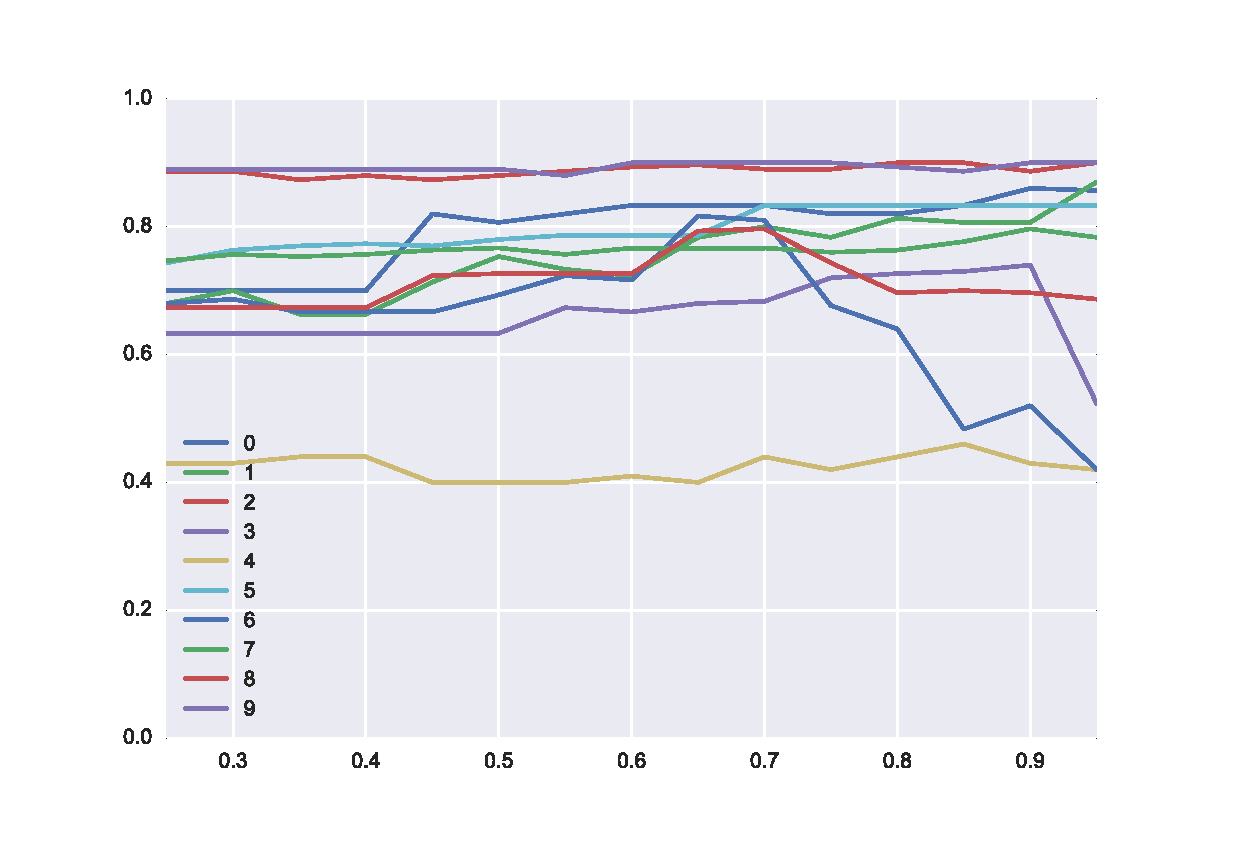
\includegraphics[height=0.22\textheight]{../figures/dim_ret_precision_line.eps}
\end{center}
\caption{Effect of diminishing returns base on precision: Doing some stuff with the DRB across sim data (branch length set).}
\label{fig:dim_rets}
\end{figure}


\subsection{Markov chain convergence}\label{subsec:markovChainConvergence}
\lipsum[3]


\subsection{Orphan placement}\label{subsec:orphanPlacement}
\begin{enumerate}
  \item Hidden Markov models are created for each individual sequence and for alignments from each cluster
  \item The probability of emitting each sequence from each sequence hmm is calculated \(forward score\)
  \item Calculate all-by-all pairwise correlation coefficients among sequences, against forward scores
  \item Create a null model from all of the R\textasciicircum2 values from pairs of sequences coming from the same RD-MCL clusters
  \item Create a truncated normal distribution between 0 and 1 for the null model
    \begin{itemize}
    \item I.e., probability that value X is randomly drawn from the population of sequence pair R\textasciicircum2 values in all clusters
    \end{itemize}
  \item Calculate the minimum R\textasciicircum2 value that will be accepted (5\%? 1\%? Use the scipy.ppf() function)
  \item
\end{enumerate}


% \subsection*{Sub-heading for section}
% Text for this sub-heading \ldots
% \subsubsection*{Sub-sub heading for section}
% Text for this sub-sub-heading \ldots
% \paragraph*{Sub-sub-sub heading for section}
% Text for this sub-sub-sub-heading \ldots
% (also see~\cite{koon,khar,zvai,xjon,marg}).
% \nocite{oreg,schn,pond,smith,marg,hunn,advi,koha,mouse}

%%%%%%%%%%%%%%%%%%%%%%%%%%%%%%%%%%%%%%%%%%%%%%
%%                                          %%
%%          Backmatter begins here          %%
%%                                          %%
%%%%%%%%%%%%%%%%%%%%%%%%%%%%%%%%%%%%%%%%%%%%%%

\begin{backmatter}

\section*{Competing interests}
  The authors declare that they have no competing interests.

\section*{Author's contributions}
  SRB is the lead developer of RD-MCL, performed all analyses unless otherwise stated, and wrote the manuscript;
  PG performed the WNT analysis;
  KEK contributed to the code base;
  and ADB was involved in the design and coordination of the project.
  All authors read and approved the final manuscript.

\section*{Acknowledgements}
  This research was supported by the Intramural Research Program of the National Human Genome Research Institute, National Institutes of Health.


%%%%%%%%%%%%%%%%%%%%%%%%%%%%%%%%%%%%%%%%%%%%%%%%%%%%%%%%%%%%%
%%                  The Bibliography                       %%
%%                                                         %%
%%  Bmc_mathpys.bst  will be used to                       %%
%%  create a .BBL file for submission.                     %%
%%  After submission of the .TEX file,                     %%
%%  you will be prompted to submit your .BBL file.         %%
%%                                                         %%
%%                                                         %%
%%  Note that the displayed Bibliography will not          %%
%%  necessarily be rendered by Latex exactly as specified  %%
%%  in the online Instructions for Authors.                %%
%%                                                         %%
%%%%%%%%%%%%%%%%%%%%%%%%%%%%%%%%%%%%%%%%%%%%%%%%%%%%%%%%%%%%%

% if your bibliography is in bibtex format, use those commands:
\bibliographystyle{bmc-mathphys} % Style BST file (bmc-mathphys, vancouver, spbasic).
\bibliography{../references/refs}      % Bibliography file (usually '*.bib' )
% for author-year bibliography (bmc-mathphys or spbasic)
% a) write to bib file (bmc-mathphys only)
% @settings{label, options="nameyear"}
% b) uncomment next line
%\nocite{label}

% or include bibliography directly:
% \begin{thebibliography}
% \bibitem{b1}
% \end{thebibliography}

%%%%%%%%%%%%%%%%%%%%%%%%%%%%%%%%%%%
%%                               %%
%% Figures                       %%
%%                               %%
%% NB: this is for captions and  %%
%% Titles. All graphics must be  %%
%% submitted separately and NOT  %%
%% included in the Tex document  %%
%%                               %%
%%%%%%%%%%%%%%%%%%%%%%%%%%%%%%%%%%%

%%
%% Do not use \listoffigures as most will included as separate files

%\section*{Figures}
% NOTE: to get the figure to stretch across both columns, use {figure*}

%%%%%%%%%%%%%%%%%%%%%%%%%%%%%%%%%%%
%%                               %%
%% Tables                        %%
%%                               %%
%%%%%%%%%%%%%%%%%%%%%%%%%%%%%%%%%%%

%% Use of \listoftables is discouraged.
%%
%\section*{Tables}

%\begin{table}[ht!]
%\caption{List of optional third party software that BuddySuite programs can interact with. BuddySuite performs all necessary format conversion to call any of these tools and, where appropriate, returns the result in the same format as the input. This is particularly useful when creating multiple sequence alignments from annotated sequences in GenBank or EMBL format.}
%      \begin{tabular}{lll}
%        \hline \\
%	   BuddySuite program	& Third-party program					& Reference  \\ \\
%        \hline
%        SeqBuddy			& BLAST 								&~\cite{Chiba:2015ed} \\
%        \hline
%        AlignBuddy			& Clustal Omega 						&~\cite{Chiba:2015ed} \\
%        					& ClustalW2 							&~\cite{Chiba:2015ed} \\
%							& MAFFT 								&~\cite{Chiba:2015ed} \\
%							& MUSCLE 								&~\cite{Chiba:2015ed} \\
%							& PAGAN 								&~\cite{Chiba:2015ed} \\
%        					& PRANK 								&~\cite{Chiba:2015ed} \\
%        \hline
%        PhyloBuddy			& FastTree 								&~\cite{Chiba:2015ed} \\
%        					& RAxML 								&~\cite{Chiba:2015ed} \\
%        					& PhyML 								&~\cite{Chiba:2015ed} \\
%        \hline
%      \end{tabular}
%\label{table:software}
%\end{table}

%%%%%%%%%%%%%%%%%%%%%%%%%%%%%%%%%%%
%%                               %%
%% Additional Files              %%
%%                               %%
%%%%%%%%%%%%%%%%%%%%%%%%%%%%%%%%%%%

%\section*{Additional Files}
%  \subsection*{Additional file 1 --- Sample additional file title}
%    Additional file descriptions text (including details of how to
%    view the file, if it is in a non-standard format or the file extension).  This might
%    refer to a multi-page table or a figure.

%  \subsection*{Additional file 2 --- Sample additional file title}
%    Additional file descriptions text.


\end{backmatter}
\end{document}
